\documentclass[00_mcda_tutorial.tex]{subfiles}

\begin{document}
\section*{Tutorial 2: effects table building}
\addtocounter{section}{1}
\addcontentsline{toc}{section}{\protect\numberline{}Tutorial 2: effects table building}

This tutorial guides you through the process of making analysable effects tables out of larger datasets.

\subsection*{Subjects covered}
\begin{itemize}
    \item Problem definition interface
    \item Creating effects tables of subsets of your measurements data
    \item Switching between effects tables
\end{itemize}

\subsection*{Example effects table}
The data that you are going to enter in this tutorial is taken from the effects table for lixisenatide as included in the \href{https://www.ema.europa.eu/documents/template-form/day-80-assessment-report-overview-d120-loq-template-guidance-rev-1019_en.docx}{EMA Guidance document for critical assessment reports} (see page 72). We use a similar table to the previous tutorial, with one more criterion and alternative.


\subsection*{Sign in to your organisation's ADDIS/MCDA.}
\leftpointright \, Open your browser and navigate to \href{https://mcda.drugis.org}{https://mcda.drugis.org}.
Use your Google account to sign in.

\begin{sidebar*}
In case of the enterprise edition, navigate to the URL provided by your organisation. Use your username and password to sign in.
\end{sidebar*}

You will be redirected to your personal homepage, containing your previously created workspaces, both finished and unfinished (if any).

\subsection*{Create a new workspace}
\leftpointright \, Press the ‘Create workspace’ button, click ‘Select tutorial workspace’, load the ‘Lixisenatide simplified’ example, and press the ‘Add’ button. This takes you to the overview screen. Take a moment to look at the criteria, alternatives, and data sources.

\subsection*{Create an analysable effects table}
\leftpointright \, Click on the ‘Problem definition’ tab. Note that the currently-selected problem (in the dropdown at the top of the screen) is the ‘Default’ problem. This problem is always automatically generated by the system and includes all criteria, alternatives, and data sources shown on the ‘Overview’ tab.
\newline

\noindent \faGraduationCap \, A ‘problem’ is our term for an analysable selection of criteria, alternatives, and data sources from those available in the workspace. This selection can include everything in the workspace, but several restrictions apply:

\begin{itemize}
    \item Only one data source can be selected per criterion
    \item No missing measurements (empty cells) are allowed for any combination of the selected criteria/alternatives
\end{itemize}

\noindent An exception is the ‘Default’ problem, which may contain multiple data sources as well as empty cells. Should this be the case, the ‘Default’ problem is considered to be not analysable, resulting in an inactive ‘Preferences’ tab. Hovering your mouse over the ‘Preferences’ tab will then show a tooltip explaining why this tab is inactive.

\noindent \leftpointright \, Click the ‘+’ icon under the ‘Problem’ dropdown (Figure \ref{fig:create_problem}). This opens the problem creation dialog.

\begin{figure}[!h]
    \centering
    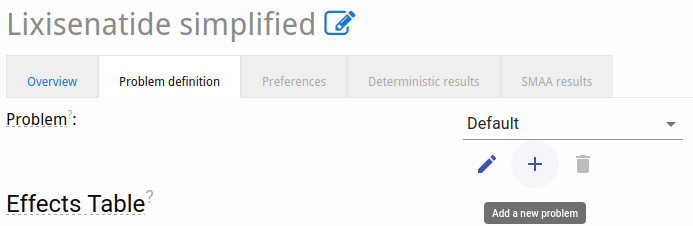
\includegraphics[width=.8\textwidth]{fig/createProblem.png}
    \caption{Problem creation button}
    \label{fig:create_problem}
\end{figure}

\noindent \leftpointright \, Scroll down and take a look at the warnings the bottom of the dialog. These explain why the current selection of criteria, alternatives, and data sources is not analysable. To make the effects table analysable, first, deselect the Exenatide criterion and then deselect the data source rows for EFC6019. This should cause the warning about missing values to disappear. Next, deselect the data source rows for EFC6015, so that we end up with a lixisenatide/placebo comparison based on pooled data EFC6014 and EFC10743 for HbA1c and Hypoglycaemia. Now the warning about multiple data sources should have disappeared (Figure \ref{fig:create_lixi_placebo}). The controls for setting the scale ranges (the breadth of possible values to asses on the ‘Preferences’ tab, see next tutorial) are now also accessible; these are not part of this tutorial. Give the problem an informative name such as ‘Lixi-PBO pooled’ and click 'Add' at the bottom of the dialog.

\begin{figure}[!h]
    \centering
    \includegraphics[width=\textwidth]{fig/createLixiPlacebo.png}
    \caption{Creating a problem}
    \label{fig:create_lixi_placebo}
\end{figure}

\noindent \leftpointright \, Observe the effects table for the new problem. Note that the ‘Preferences’ tab has now become enabled. That tab and the ones to its right are the subject of the following tutorials.

\subsection*{Create more effects tables}
\noindent \leftpointright \, Create another problem, this time selecting EFC6015 as data source for HbA1c and Hypoglycaemia, and indicate this fact in the title.
\newline

\noindent \faLightbulbO \, When creating a new problem, the initially-selected criteria and alternatives are based on those of the current problem. The initial ‘Default’ problem always has everything selected, and thus may not be usable for analysis.
\newline

\noindent \leftpointright \, Create another problem, but now to compare Lixisenatide and Exenatide. Note that, since there is no data source with measurements for Nausea for both alternatives, this problem must omit Nausea as a criterion.
\newline

\noindent \leftpointright \, Use the ‘Problem’ dropdown at the top of the tab to switch between your effects tables. Observe that the effects table and browser URL changes whenever you switch problem.
\newline

\noindent \faGraduationCap \, Creating a set of problems that all look at different aspects of your workspace’s data lets you contrast the alternatives in different ways. For each problem you can then define a further set of scenarios with different preferences regarding the importance of your criteria, and compare their benefit-risk balances (subject of the next tutorial).

\subsection*{Workspace and view settings}

\noindent \leftpointright \, Click on the ‘settings’ button at the top of the tab (Figure 3). This lets you customise your view of the effects table and measurements in general. Take a moment to study the different settings you can choose. Play with the top three settings by changing their value and clicking ‘Save’, and observe the results. What should happen:

\begin{itemize}
    \item Changing to Median/Mode does nothing (this only applies when the values shown in the effects table are sampled from probability distributions).
    \item Changing the ‘Measurements display mode’ from ‘Entered effects’ to ‘Values used in deterministic analysis’ shows the values as they will be used for calculating the deterministic results.
          Changing to ‘Entered distributions’ shows the distributions and their parameters used for calculating the SMAA results. For this example no distributions where entered and this option is not availbable.
    \item Changing to ‘Values used in SMAA’ shows the 95\% confidence interval calculated from the distributions, however since we’ve only entered effects for this example, it will show the point estimate of those effects.
    \item Changing between percentages and decimals changes the shown values and units for Nausea and Hypoclycaemia but not HbA1c (this setting only affects dichotomous criteria).
\end{itemize}

\noindent \leftpointright \, Uncheck e.g. the ‘Description’ and ‘Uncertainties / Strength of evidence’ checkboxes in the bottom section of the settings dialog to make the effects table more compact. Click ‘Save’ and study the result.

\subsection*{Export effects table}
\noindent \leftpointright \, Open a rich text editor, such as MS Word, LibreOffice or Google Docs. Choose one of your effect tables, and click the ‘Copy to clipboard’ button (Figure \ref{fig:clipboard_button}). Now go to the editor and paste the selection in there. This should result in a structured table similar to the one in the browser. Depending on your editor and its settings, you may want to adjust things like whether there are borders around cells in your editor’s table settings.

\begin{figure}[!h]
    \centering
    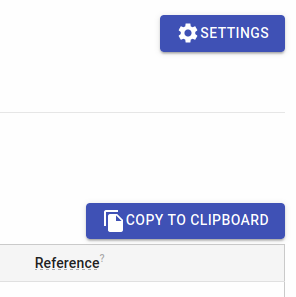
\includegraphics[width=.5\textwidth]{fig/clipboardButton.png}
    \caption{Settings and copy buttons}
    \label{fig:clipboard_button}
\end{figure}

\subsection*{Final words}
We hope that this tutorial has demonstrated adequately how to go from a wider data set to a smaller effects table that can be used to analytically study the benefit-risk balance of selected alternatives for selected criteria. We’ve also shown how to switch between such problems at will. Finally, we’ve shown how to change several aspects of how the effects table is displayed, and how to export your effects table to text editors e.g. for report writing.

\end{document}